\subsection{Drift detection}
    Assume that during training labeled data comes from a distribution $p$, meaning $\{(x^{(1)}, y^{(1)}), ..., (x^{(n)}, y^{(n)})\} \sim p$ and during deployment unlabeled data comes from a distribution $q$, meaning $\{x^{(1)}\prime, ..., x^{(1)}\prime\} \sim q$. The goal of the drift detection is to determine if $q(x\prime)$ is the same data distribution as $p(x)$. Or, putting it more formally, determine which hypothesis holds: null-hypothesis $H_0$ and an alternative hypothesis $H_A$, where $H_0:p(x) = q(x)$ and $H_A:p(x) \neq q(x)$.

    Having samples from both distributions or representation of these samples in lower dimension, one can then choose a statistical hypothesis test to compare these distributions (\cite{Muandet_2017}).
    \subsubsection{Drift detection vs. outliers detection}
        After developement phase when model training is finished, the model will be moved into a deployment or a production, where it is supposed to maintain an expected quality of predictions. However input data is not always a stable source of input. One should constantly maintain quality of predictions and do a regular check-ups for outliers as well as to alert an end-user about a drift in input data. Drift detection happens on raw data in absence of the ground truth labels and serves as a signal that the input data differs a lot from the data used for training, meaning that predictions became not reliable.

There is a significant difference between distinguishing drift of the whole source of data in comparison to detecting single outliers. In drift detection, one looks at the whole new input data as a distribution and checks if there is a significant shift in comparison to the data used during training.

There are two possible reactions after the drift is detected: alert the user that predictions became unreliable, and therefore she should consider expanding the dataset by adding more labeled data from a new drifted distribution in training or apply some different logic on the model outputs. When an outlier is detected, a model might request human assistance for some particular input, because this input is too unfamiliar to the model and possibly it won't give a good prediction on this one.

The goal of outlier detection is to decide on the single instances whether or not it is different from training data or unusual in some way or another. Outliers might appear both in training and prediction datasets.

Data drift and outlier detection can co-exist. It might be that the input is drifted, but there are no outliers, it might be that there are a lot of outliers, but the data was not drifted. (\cite{samuylova_2021}).

Important observation here is that the drift detector should be robust to outliers. The system should not send an alert as soon as it sees a suspicious sample due to the fact that outlier might be present in the original data distribution as well. But the alert should happen when there are many such samples. To compare original training data distribution and the new one from inputs different statistical tests like Kolmogorov-Smirnov, Chi-squared and etc. can used.

The need of maintaining drift detection or outlier detection depends on the costs on the errors. If the cost of a single error is too high, one should use an outlier detection, but when one needs a test to decide when to label new data - drift detection would be a better approach.

In summary, the drift detection is needed only when the meaningful shifts of the input data distribution from the training distribution need to be detected, whereas the outlier detector aims at finding unusual single instances in inputs. Here this is exactly the case, we train models assuming correct set up  of microscopy image acquisition, however changes in exposure, illumination, cell fixation procedure might alternate DIC imaging. In this case user has to be informed about it and choose afterwards whether he wants to add more data to the training set or not to use model's predictions.

    \subsubsection{Kernel methods and two-sample testing}
        The test used in this work for determinig wether two distributions are the same or not is one of the multivariate kernel two-sample tests and called Maximum Mean Discrepancy or shotly MMD. The idea behid any two-sample testing is to choose two random samples, where each was taken from one of the two different distributions and afterwards to decide wether the difference in them is statistically significant. 

MMD is a kernel-based method that can distinguish between two distributions based on their kernel mean embeddings  in a reproducing kernel Hilbert space (RKHS) (\cite{Rabanser_2018}).

The idea behind a Hilbert space embedding distribution (or a kernel mean embedding) is to map a distribution into a point in a reproducing Hilbert space. After this step, one is allowed to use all powerful kernel methods for probability measures, resulting in methods like kernel two-sample testing. One of the widely known kernel methods if a support vector machines (SVM).

To understand why kernel mean embeddings are so successful one has to first understand what a kernel function is. With the help of kernel functions an inner product of elements $x, y \in \mathcal{X}$ in some high-dimensional feature space can be calculated. If kernel function is positive definite, then there always exists a dot product space $\mathscr{H}$ along with a function that maps a space $\mathcal{X}$ into space $\mathscr{H}$: $\phi : \mathcal{X} \rightarrow \mathscr{H}$ such that $k(x, y) = {\langle\phi(x), \phi(y)\rangle}_{\mathscr{H}}$ and most importantly there is no need for explicit computation of $\phi$ (\cite{Smola_2002}). Therefore if there exists an algorithm that can be expressed through dot product of $\langle x, y \rangle$ then kernel function can be applied to this dot product and this is called a \textit{kernel trick} (\cite{Smola_2002}).

Now, kernel mean embedding actually extends the above mentioned feature map $\phi$ to the space of probability distributions. In this space each probability distribution will be mapped to a mean function defined as follows:

\begin{equation}
    \phi(\mathds{P}) = \mu_{\mathds{P}} := \int_{\mathcal{X}}k(x, \cdot)d\mathds{P}(x)
\end{equation}

Here $k(x, \cdot)$ is a positive definite symmetric kernel function. Main goal here is to map a distribution $\mathds{P}$ to an point in the feature space $\mathscr{H}$ and this feature space is exactly an RKHS that corresponds to a kernel $k$. Such a mapping might be useful because it captures all information about the initial distribution $\mathds{P}$. This mapping $\mathds{P} \rightarrow \mu_\mathds{P}$ is injective. This means that $||\mu_\mathds{P} - \mu_\mathds{Q}||_{\mathscr{H}} = 0$ if and only if $\mathds{P} = \mathds{Q}$. Here it means that $\mathds{P}$ and $\mathds{Q}$ is the same distribution. Additionally since the mapping is injective, it is possible to use such characterization of a distribution to be used in two-sample homogenneity tests, which is exactly what is needed here. 

To estimate a kernel mean embedding is much easier than to estimate a distribution itself. This approach is successfully used in data-generating processes, it also improves some statistical inference methods like two-sample testing. Such approach is also useful when instead of data points in testing and training datasets there are probability distributions. 

Inner product $\langle x, y \rangle$ can be viewed as a similarity measure between $x$ and $y$. This inner product includes a class of linear functions and this class is too restrictive for many applications, however there is a simple possible extension to add non-linearities to it with the mapping: \begin{equation}
    \phi: \mathcal{X} \rightarrow \mathcal{F}
\end{equation} where \begin{equation}
    \phi: x \rightarrow \phi(x)
    \label{equation:positive-definite}
\end{equation}

Here $\mathcal{F}$ is high-dimensional feature space and it is possible to evaluate then:

\begin{equation}
    k(x, y) := {\langle\phi(x), \phi(y)\rangle}_{\mathcal{F}}
\end{equation} with  ${\langle \cdot, \cdot \rangle}_{\mathcal{F}}$ denoting an inner product in of $\mathcal{F}$.

Now $ k(x, y)$ is already a non-linear similarity measure between $x$ and $y$. In order to get a non-linear version of the algorithms that use dot product simply sustitute $\langle x, y\rangle$ with $ {\langle\phi(x), \phi(y)\rangle}_{\mathcal{F}}$. 

Let's define the following mapping that represents in $\mathcal{X}$ any probability measure $\mathds{P}$ and denote it as $\mu_{\mathds{P}}$. This mapping is called a kernel mean embedding.

\begin{definition}[Kernel mean embedding]
    cite Berlinet and Thomas Agnan 2004
    The kernel mean embedding of probability measure in $M^1_+(\mathcal{X})$ into RKHS $\mathscr{H}$ endowed with a reproducing kernel $k: \mathscr{H} \times \mathscr{H} \rightarrow \mathds{R}$ is defined by a mapping 
    \begin{equation}
        \mu : M^1_+(\mathcal{X}) \rightarrow \mathscr{H}, \mathds{P} \rightarrow \int k(x, \cdot)d\mathds{P}(x)
    \end{equation}
\end{definition}

However, usually there is no access to the distribution $\mathds{P}$ and that is why one cannot directly compute $\mu_{\mathds{P}}$. Fortuntel, there are samples that can be drawn from this distribution and with their use one can make a good approximation of $\hat{\mu}_{\mathds{P}}$ of a true kernel mean embedding $\mu_{\mathds{P}}$. One of such approximations could be the following unbiased estimate:
\begin{equation}
    \hat{\mu}_{\mathds{P}} := \frac{1}{n} \sum_{i=1}^n k(x_i, \cdot)
\end{equation}

Moreover, this estimator $\hat{\mu}_{\mathds{P}}$  will converge to $\mu_{\mathds{P}}$ by the law of large numbers as $n \rightarrow \infty$.

\begin{definition}[Characteristic kernel]
    A kernel $k$ is a characteristic kernel if the map $\mu: \mathds{P} \rightarrow \mu_{\mathds{P}}$ is injective. If the reproducing kernel of the RKHS $\mathscr{H}$ is characteristic, then RKHS is called characteristic as well. 
\end{definition}

In machine learning applications and statistics kernel mean embedding is as a metric for the probability distributions. And mean embeddings metric is actually just a specific case of a more general so-called integral probability metric (IPM) (\cite{Mueller_1997}).

\begin{definition}[IPM]
    Let $\mathds{P}$ and  $\mathds{Q}$ be two probability measures on some measurable space $\mathcal{X}$. Then IPM is defined as follows:
    \begin{equation}
        \gamma [\mathcal{F}, \mathds{P}, \mathds{Q}] = \sup_{f\in \mathcal{F}} \left\{ \int f(x) d\mathds{P}(x) -  \int f(y) d\mathds{Q}(y) \right\}
    \label{eq:ipm}
    \end{equation}
    with $\mathcal{F}$ being a space of real-value bounded functions.
\end{definition}
    \subsubsection{Maximum mean discrepancy for drift detection}
        \begin{figure}[H]
	\begin{center}
		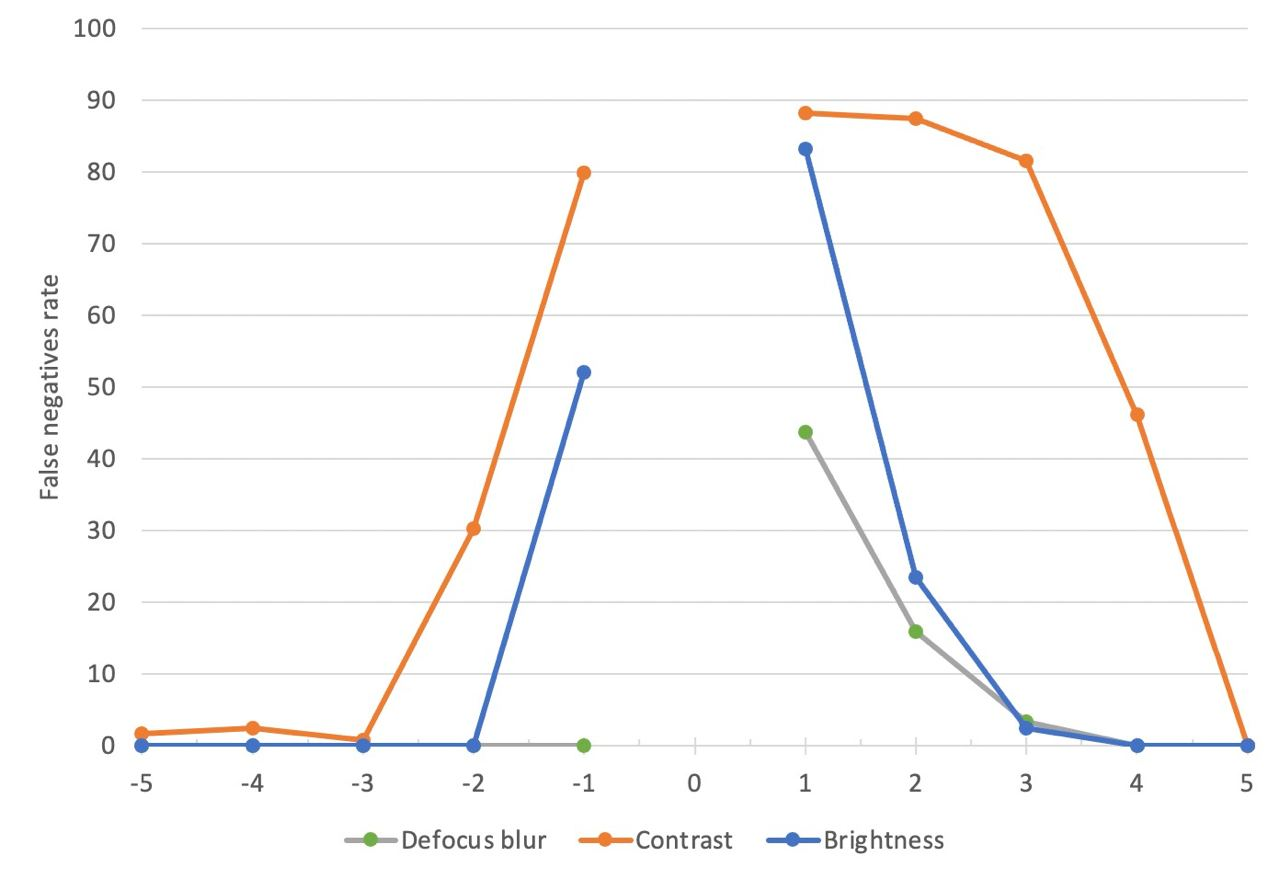
\includegraphics[width=0.5\linewidth]{bilder/drift-detection/fn-rate.jpg}
		\caption{False negatives rate for drift detection on artificial corruptions}\label{fig:fn-rate}
	\end{center}
\end{figure}
    \subsubsection{Drift detection experiments}
        \begin{figure}[H]
	\begin{center}
		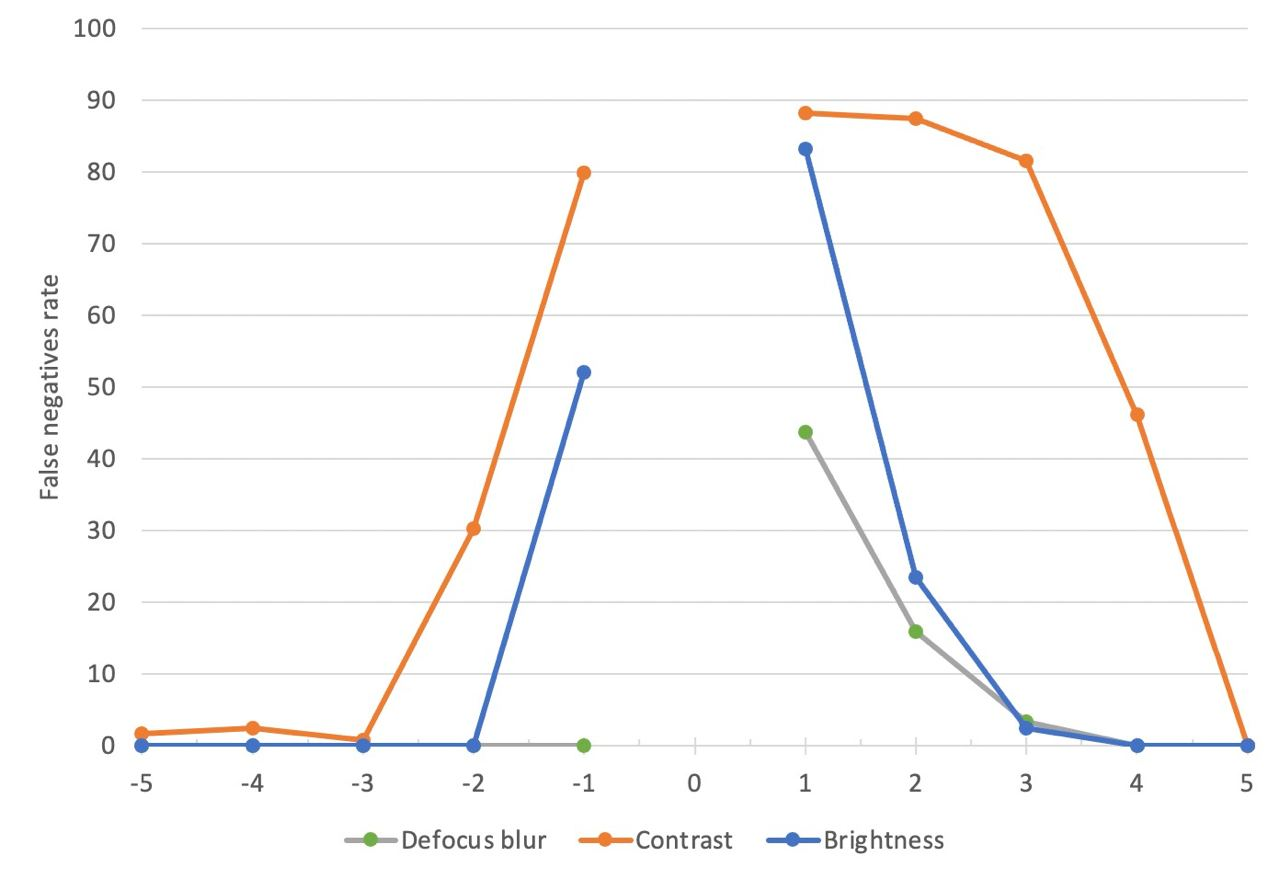
\includegraphics[width=0.5\linewidth]{bilder/drift-detection/fn-rate.jpg}
		\caption{False negatives rate for drift detection on artificial corruptions}\label{fig:fn-rate}
	\end{center}
\end{figure}
    \subsubsection{Online drift detection experiments}
            MMD algorithm in \textit{alibi-detect} library has an online version, which also presents an interest for our case. One of the main differences of an online drift detector is that it does not accept several inputs at once alerting whether they represent a drift all together, but it focuses on a single input at a time during its run. It assumes that there is a big dataset of reference data, that can be used as an example of a "correct" distribution and processes one embedding at a time. This single input would be sent into a test window where two-sample test-statistics (MMD essentially in this case) will be calculated. As soon as the test-statistic exceeds some pre-defined threshold a drift alert is send to the user. Apart from the threshold one has to define a so-called expected run-time (ERT). This time states how many inputs the detector should process on average before it makes a detection (false positive or true positive depending on which distributions the inputs were taken from). Another hyperparameter here is hidden in a size of a test-window. Becase the larger the window is, the more chance is there to detect a very slight drift, yet with a smaller window one gets a much faster response to severe drift. 

It is usually recommened to reduce the dimensionality of the data before feeding it into the algorithm. But in this case the performance was exceptional even for high-dimensional embeddings of the UNET model. Nevertheless, there are also options on how to reduce the dimensionality of the data from the authors of the framework.

This algorithm was trained on the same uncorrupted training data sent through the embeddings of a nucleus UNet. Yet, test crops are fed into a detector in a consecutive way --- in case of no corruptions present it is not enough to feed only several crops from one image, as the algorithm requires more data to be fed into the detector until it makes a decision. For example, ERT of not corrupted inputs can be even up to $180$ crops until a detector alerts a false positive detection. On the contrary for corrupted inputs drift detector needs normally $\leq 6$ crops (see Figure \ref{fig:online-ert})
\begin{figure}[H]
	\begin{center}
		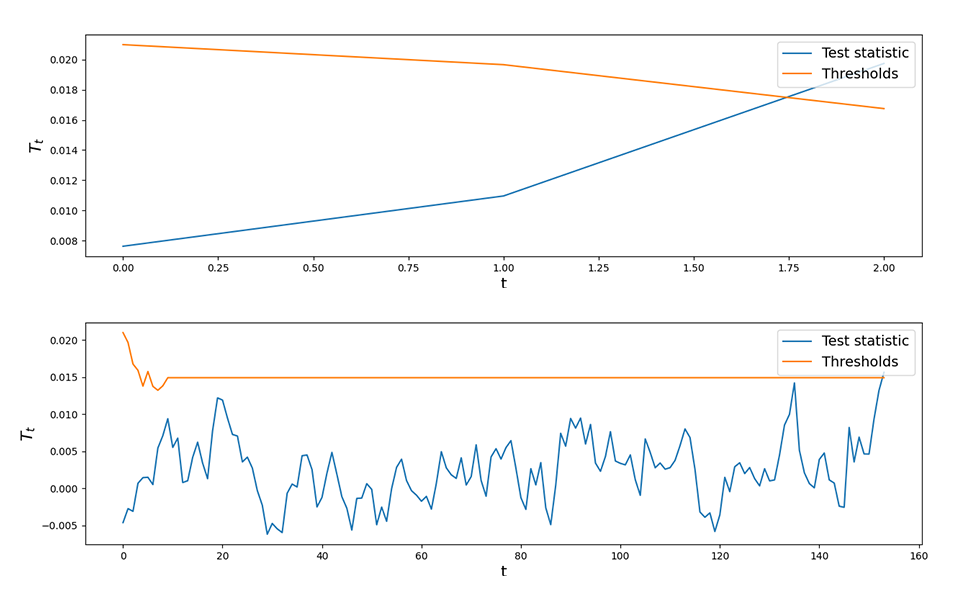
\includegraphics[width=0.6\linewidth]{bilder/drift-detection/online.png}
		\caption{Expected runtime (ERT) for corrupted and in-distribution data}\label{fig:online-ert}
	\end{center}
\end{figure}

Having such a detector one measures ERTs for not corrupted inputs, then for corrupted ones and afterwards calculates the best threshold that can separate the two. ERTs of corrupted data should be much lower than ERTs of not corrupted one. In this experiment ERTs of both classes were separable, however both located very close to the threshold: $\approx 4.59$ for corrupted ones and $\approx 7.1$ for not corrupted. Yet with a threshold of $6$ the accuracy scores are very high. Having a drift detector trained on not corrupted training data only, one can estimate ROC-AUC scores between two classes: not corrupted test data and the same test data but with some corruption applies to it. The results of this experiment with a defocus blur corruption of several severities are presented in Figure \ref{fig:online-auc-roc}. Already on severity 3, such detector separates the two almost perfectly. The scores are also presented in Table \ref{tab:severity-separability}.

\begin{figure}[htb]
	\begin{center}
		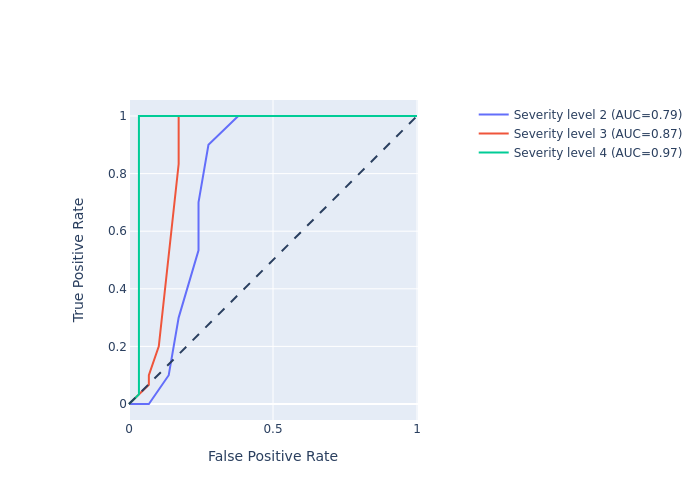
\includegraphics[width=0.8\linewidth]{bilder/drift-detection/auc_roc comparison online.png}
		\caption{AUC ROC scores for various defocus corruption severities}\label{fig:online-auc-roc}
	\end{center}
\end{figure}

\begin{table}[htb]
    \centering
    \caption{Severity of corruptions on separability}
        \begin{adjustbox}{width=0.4\textwidth}
            \begin{tabular}{|l||*{3}{c|}}\hline
                \makebox{W}
                &\makebox[3em]{Level 2}
                &\makebox[3em]{Level 3}
                &\makebox[3em]{Level 4}
                \\\hline\hline
                Auc-Roc &0.84&0.92&0.98\\\hline
            \end{tabular}
            \label{tab:severity-separability}
        \end{adjustbox}
\end{table}

Additionally, research has been performed on the influence of the hyperparameters to an online MMD drift detector, specifically: test window size, specified ERT. The results are presented in Tables \ref{tab:test-window-size-influence}, \ref{tab:ert-influence}. Test window size influences how fast and how sensitive the reaction of an algorithm should be and the ideal value in this case would be $10$ crops, during this time a threshold will be established. In case of ERT as a hyperparameter as long as it is big enough the score does not change very much.

\begin{table}[H]
    \centering
    \caption{Test window size influence on separability}
        \begin{adjustbox}{width=0.6\textwidth}
            \begin{tabular}{|l||*{5}{c|}}\hline
                \makebox{W}
                &\makebox[3em]{2}
                &\makebox[3em]{5}
                &\makebox[3em]{10}
                &\makebox[3em]{15}
                &\makebox[3em]{20}
                \\\hline\hline
                Auc-Roc &0.85&0.92&0.98&0.90&0.88\\\hline
            \end{tabular}
            \label{tab:test-window-size-influence}
        \end{adjustbox}
\end{table}

\begin{table}[H]
    \centering
    \caption{ERT influence on separability}
        \begin{adjustbox}{width=0.5\textwidth}
            \begin{tabular}{|l||*{4}{c|}}\hline
                \makebox{W}
                &\makebox[3em]{32}
                &\makebox[3em]{64}
                &\makebox[3em]{128}
                &\makebox[3em]{256}
                \\\hline\hline
                Auc-Roc &0.90&0.95&0.98&0.98\\\hline
            \end{tabular}
            \label{tab:ert-influence}
        \end{adjustbox}
\end{table}

            \paragraph{Impact of cell fixation}
                In section \ref{section:gfp} the difference between fixed and not fixed cells was mentioned. Visual analysis of model's predictions for not fixed cells after training it on fixed ones has shown that the model was not able to generalize well on them. This is the reason why it would be important to alarm the end user to not rely on predictions when such a situation occurs. In this case an online drift detector trained using not corrupted data used for ER training first and tested on not fixed ER cells. The results of this test are shown in Figure \ref{fig:online-drift-not-fixed}.
                \begin{figure}[htb]
                    \begin{center}
                        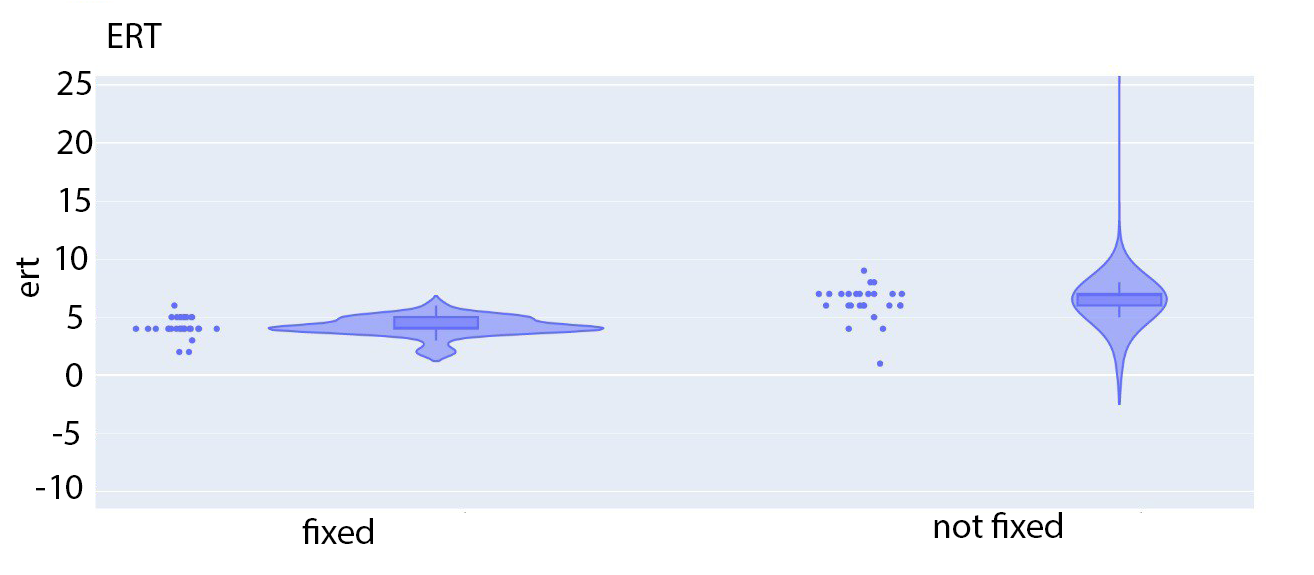
\includegraphics[width=0.5\linewidth]{bilder/drift-detection/online-fixed-vs-not-fixed.png}
                        \caption{Online drift detection of not fixated cells}\label{fig:online-drift-not-fixed}
                    \end{center}
                \end{figure}
                The ERTs for corrupted data (left) are lower from ERT for true input. The ROC-AUC score for the separability is $0.91$ and the best threshold is $6$. However, not corrupted data (fixed cells) mostly have an ERT of $7$, whereas corrupted data (not fixed cells) have an ERT of $4$. Both classes have ERTs that are very close to the threshold, but are able to separate the classes well enough.

                Application of a usual drift detection algorithm with the use of ER model the false positive rate on not corrupted (fixed) cells was $0.075$. Whereas all fixed cells were recognized as drift.  